% ----------------------------------------------------
% ----------------------------------------------------
% Implementation
% ----------------------------------------------------
\documentclass[class=report,11pt,crop=false]{standalone}
% Page geometry
\usepackage[a4paper,margin=20mm,top=25mm,bottom=25mm]{geometry}

% Font choice
\usepackage{lmodern}

\usepackage{lipsum}

% Use IEEE bibliography style
\bibliographystyle{IEEEtran}

% Line spacing
\usepackage{setspace}
\setstretch{1.2}

% Ensure UTF8 encoding
\usepackage[utf8]{inputenc}

% Language standard (not too important)
\usepackage[english]{babel}

% Skip a line in between paragraphs
\usepackage{parskip}

% For the creation of dummy text
\usepackage{blindtext}

% Math
\usepackage{amsmath}

% Header & Footer stuff
\usepackage{fancyhdr}
\pagestyle{fancy}
\fancyhead{}
\fancyhead[R]{\nouppercase{\rightmark}}
\fancyfoot{}
\fancyfoot[C]{\thepage}
\renewcommand{\headrulewidth}{0.0pt}
\renewcommand{\footrulewidth}{0.0pt}
\setlength{\headheight}{13.6pt}

% Epigraphs
\usepackage{epigraph}
\setlength\epigraphrule{0pt}
\setlength{\epigraphwidth}{0.65\textwidth}

% Colour
\usepackage{color}
\usepackage[usenames,dvipsnames]{xcolor}

% Hyperlinks & References
\usepackage{hyperref}
\definecolor{linkColour}{RGB}{77,71,179}
\definecolor{urlColour}{RGB}{255, 179, 102}

\hypersetup{
    colorlinks=true,
    linkcolor=linkColour,
    filecolor=linkColour,
    urlcolor=urlColour,
    citecolor=linkColour,
}
\urlstyle{same}

% Automatically correct front-side quotes
\usepackage[autostyle=false, style=ukenglish]{csquotes}
\MakeOuterQuote{"}

% Graphics
\usepackage{graphicx}
\graphicspath{{Figures/}{../Figures/}}
\usepackage{makecell}
\usepackage{transparent}
\usepackage{pgfplots}
\pgfplotsset{compat=newest}
%% the following commands are needed for some matlab2tikz features
\usetikzlibrary{plotmarks}
\usetikzlibrary{arrows.meta}
\usepgfplotslibrary{patchplots}
\usepackage{float}

% Tables
\usepackage{multirow} 
\usepackage{colortbl}

% SI units
\usepackage{siunitx}

% Microtype goodness
\usepackage{microtype}

% Listings
\usepackage[T1]{fontenc}
\usepackage{listings}
\usepackage[scaled=0.8]{DejaVuSansMono}

% Custom colours for listings
\definecolor{backgroundColour}{RGB}{250,250,250}
\definecolor{commentColour}{RGB}{73, 175, 102}
\definecolor{identifierColour}{RGB}{196, 19, 66}
\definecolor{stringColour}{RGB}{252, 156, 30}
\definecolor{keywordColour}{RGB}{50, 38, 224}
\definecolor{lineNumbersColour}{RGB}{127,127,127}
\lstset{
  language=Matlab,
  captionpos=b,
  aboveskip=15pt,belowskip=10pt,
  backgroundcolor=\color{backgroundColour},
  basicstyle=\ttfamily,%\footnotesize,        % the size of the fonts that are used for the code
  breakatwhitespace=false,         % sets if automatic breaks should only happen at whitespace
  breaklines=true,                 % sets automatic line breaking
  postbreak=\mbox{\textcolor{red}{$\hookrightarrow$}\space},
  commentstyle=\color{commentColour},    % comment style
  identifierstyle=\color{identifierColour},
  stringstyle=\color{stringColour},
   keywordstyle=\color{keywordColour},       % keyword style
  %escapeinside={\%*}{*)},          % if you want to add LaTeX within your code
  extendedchars=true,              % lets you use non-ASCII characters; for 8-bits encodings only, does not work with UTF-8
  frame=single,	                   % adds a frame around the code
  keepspaces=true,                 % keeps spaces in text, useful for keeping indentation of code (possibly needs columns=flexible)
  morekeywords={*,...},            % if you want to add more keywords to the set
  numbers=left,                    % where to put the line-numbers; possible values are (none, left, right)
  numbersep=5pt,                   % how far the line-numbers are from the code
  numberstyle=\tiny\color{lineNumbersColour}, % the style that is used for the line-numbers
  rulecolor=\color{black},         % if not set, the frame-color may be changed on line-breaks within not-black text (e.g. comments (green here))
  showspaces=false,                % show spaces everywhere adding particular underscores; it overrides 'showstringspaces'
  showstringspaces=false,          % underline spaces within strings only
  showtabs=false,                  % show tabs within strings adding particular underscores
  stepnumber=1,                    % the step between two line-numbers. If it's 1, each line will be numbered
  tabsize=2,	                   % sets default tabsize to 2 spaces
  %title=\lstname                   % show the filename of files included with \lstinputlisting; also try caption instead of title
}

% Caption stuff
\usepackage[hypcap=true, justification=centering]{caption}
\usepackage{subcaption}

% Glossary package
% \usepackage[acronym]{glossaries}
\usepackage{glossaries-extra}
\setabbreviationstyle[acronym]{long-short}

% For Proofs & Theorems
\usepackage{amsthm}

% Maths symbols
\usepackage{amssymb}
\usepackage{mathrsfs}
\usepackage{mathtools}

% For algorithms
\usepackage[]{algorithm2e}

% Spacing stuff
\setlength{\abovecaptionskip}{5pt plus 3pt minus 2pt}
\setlength{\belowcaptionskip}{5pt plus 3pt minus 2pt}
\setlength{\textfloatsep}{10pt plus 3pt minus 2pt}
\setlength{\intextsep}{15pt plus 3pt minus 2pt}

% For aligning footnotes at bottom of page, instead of hugging text
\usepackage[bottom]{footmisc}

% Add LoF, Bib, etc. to ToC
\usepackage[nottoc]{tocbibind}

% SI
\usepackage{siunitx}

% For removing some whitespace in Chapter headings etc
\usepackage{etoolbox}
\makeatletter
\patchcmd{\@makechapterhead}{\vspace*{50\p@}}{\vspace*{-10pt}}{}{}%
\patchcmd{\@makeschapterhead}{\vspace*{50\p@}}{\vspace*{-10pt}}{}{}%
\makeatother

% Wrap figure
\usepackage{wrapfig}
\makenoidxglossaries

\newacronym{af}{AF}{Autofocus}
\newacronym{cli}{CLI}{Command-line Interface}
\newacronym{cpi}{CPI}{Coherent Processing Interval}
\newacronym{cptwl}{CPTWL}{Coherent Processing Time Window Length}
\newacronym{cw}{CW}{Continuous Waveform}
\newacronym{ds}{DS}{Dominant Scatterer}
\newacronym{dsa}{DSA}{Dominant Scatterer Algorithm}
\newacronym{sdsaf}{SDSAF}{Single Dominant Scatterer Autofocus}
\newacronym{fft}{FFT}{Fast Fourier Transform}
\newacronym{fmcw}{FMCW}{Frequency Modulated Continuous Waveform} % Not sure
\newacronym{hrr}{HRR}{High Resolution Range}
\newacronym{hrrp}{HRRP}{High Resolution Range Profile}
\newacronym{ic}{IC}{Image Contrast}
\newacronym{isar}{ISAR}{Inverse Synthetic Aperture Radar}
\newacronym{jtf}{JTF}{Joint Time-Frequency}
\newacronym{pri}{PRI}{Pulse Repetition Interval}
\newacronym{prf}{PRF}{Pulse Repetition Frequency}
\newacronym{qlp}{QLP}{Quick-look Processor}
\newacronym{ra}{RA}{Range Alignment}
\newacronym{rlos}{RLOS}{Radar Line of Sight}
\newacronym{rmc}{RMC}{Rotational Motion Compensation}
\newacronym{sfw}{SFW}{Stepped Frequency Waveform}
\newacronym{sf}{SF}{Scaling Factor for Haywood Autofocus}
\newacronym{sar}{SAR}{Synthetic Aperture Radar}
\newacronym{snr}{SNR}{Signal-to-Noise Ratio}
\newacronym{sir}{SIR}{Signal-to-Interference Ratio}
\newacronym{tmc}{TMC}{Translational Motion Compensation}


\begin{document}
\ifstandalone
\tableofcontents
\fi
% ----------------------------------------------------
\chapter{Quick-look Processor design \label{ch:QLPdesign}}

% ----------------------------------------------------
% Characteristics of the design section
% •	When developing a new system, ensure that you have user requirements, technical requirements and acceptance test procedures 
% •	Clear motivations provided in selecting the approach used to solve the problem stated in the introduction 
% •	Diagrams to aid the documentation of the design: block diagram, UML diagrams, circuit diagrams, flow charts, pseudo-code 
% •	Clarifying the interfaces between components 
% •	When a design decision needs to be made, multiple options are identified before a decision is made with logical reason(s) 
% •	Meticulous attention to detail in the design description  
% •	Design considers testing done to evaluate the system in the implementation phase (test points on a PCB, RF coupler in RF design)

% Characteristics of the practical work section: implementation, simulation
% •	Practical work done was relevant. Quantity and quality of the work was suitable for the degree 
% •	Document how you captured experimental data. Include photos of experimental environment and equipment used. Record details of equipment configuration, calibration procedures. 
% •	Document sub-systems were tested and evaluate if technical specifications were met
% •	Document system testing and evaluate if technical specifications were met 

 % Characteristics of the results section:  analysis of measured data and interpretation of results
% •	Clear, logical, relevant, and accurate analysis of the data and interpretation of results 
% •	Important features of the data are highlighted to the reader. 
% •	The logical conclusions from the interpretations of the data are linked to the research objectives/questions of the work 
% •	Includes a discussion on how results in this work are similar or different to results presented in the literature. If similar, state reasons why its similar. If different, explain reasons for differences. Simply saying the results are similar or different is not sufficient. 
 
% Important elements when presenting graphs in your work
% •	Explain the axes of the graph 
% •	Identify the portion of the graphs that are important. Consider annotating your graphs to ease this process
% •	Interpret what the graph means in the context of your work

\emph{Chapter introduction: Clear motivations provided in selecting the approach used to solve the problem}

\section{Technical Requirements}

\begin{table}[H]
    \centering
    \resizebox{\linewidth}{!}{%
        \begin{tabular}{|c|l|}
            \hline
            \textbf{Number}  & \textbf{Description} \\
            \hline
            TR01 & The \gls{qlp} should process the data in a shorter time than the measurement time of the data.  \\
            \hline
            TR02 & The \gls{qlp} should produce a more focused \gls{isar} image after motion compensation. \\
            \hline
            TR03 & The \gls{qlp} should be user-friendly.\\
            \hline
        \end{tabular}
    }
    \caption{Technical requirements considered when designing the \gls{qlp}.}
    \label{tab:technical_requirements}
\end{table}

%%%%%%%%%%%%%%%%%%%%%%%%%%%%%%%%%%%%%%%%%%%%%%%%%%%%%%%%%%%%%%%%%%%%%%%%%%%%%%%%%%%%%%%%
\section{Design Implementation}
\begin{figure}[H]
    \centering
    \resizebox{0.95\linewidth}{!}{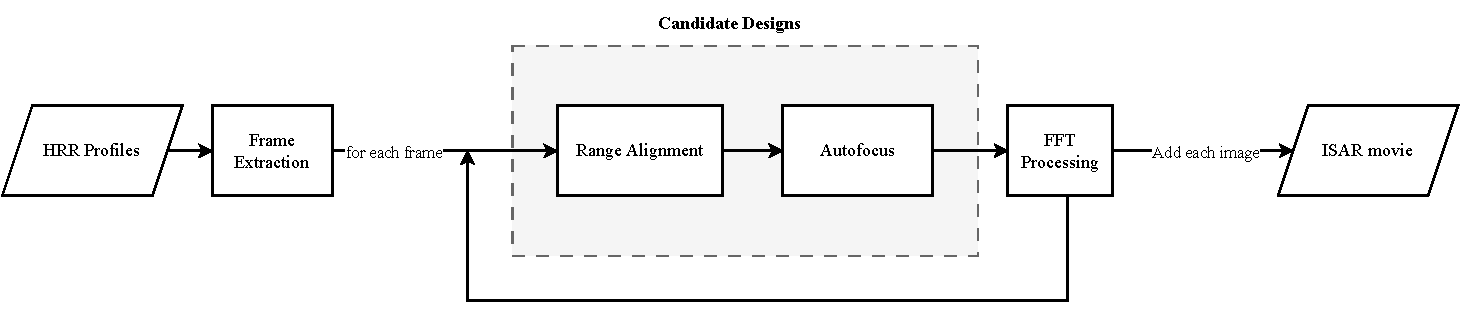
\includegraphics{Figures/05QLPDesign/FlowCharts/CandidateQLPDesigns.pdf}}
    \caption{Caption}
    \label{fig:enter-label}
\end{figure}
    %***************************************************************************************
    \subsection{Frame Extraction}
        \begin{itemize}
            \item explain why needed and CPTWL value
            \item pseudo code
        \end{itemize}

    %***************************************************************************************
    \subsection{Algorithms}
    The \gls{ra} and \gls{af} algorithms that were validated and verified in \autoref{ch:algorithmV&V} were considered for use in the final \gls{qlp}. The four candidate designs are listed in \autoref{tab:candidate_qlp_designs}. 
        \begin{table}[H]
            \centering
            \begin{tabular}{|c|l|l|}
                \hline
                \textbf{Candidate Design} & \textbf{\gls{ra} Algorithm} & \textbf{\gls{af} Algorithm}\\
                \hline
                 1  &  Correlation    & Single Dominant Scatterer\\
                 \hline
                 2  &  Correlation    & Single Dominant Scatterer\\
                 \hline
                 3  &  Haywood        & Multiple Dominant Scatterer\\
                 \hline
                 4  &  Haywood        & Multiple Dominant Scatterer\\
                 \hline
            \end{tabular}
            \caption{Candidate \gls{qlp} Designs}
            \label{tab:candidate_qlp_designs}
        \end{table}

    To determine the most suitable candidate design, all designs were validated against the respecrequirements and specifications in tables \autoref{tab:requirements} and \autoref{tab:specifications}.
    
\section{Experimental Setup}

    %***************************************************************************************
    \subsection{Runtime Testing}
    A \textsc{MATLAB} \href{}{timing script} was used to measure the runtime of each candidate \gls{qlp} design. The script was used to run each candidate design 100 times and the raw timing results were recorded in a CSV file. The timing tests were performed using a single measured dataset. A folder containing the testing files is available on \href{}{GitHub}.

    The testing was conducted on a MacBook Pro (2016) with the following hardware specifications:
    \begin{itemize}
        \item Processor: 2.9GHz Dual-Core Intel Core i5
        \item Memory: 8GB 2133MHz LPDDR3
    \end{itemize}

    %***************************************************************************************
    \subsection{Image Contrast Testing}
    
\section{Results and Discussion}
    %***************************************************************************************
    \subsection{Runtime Testing}
    The raw timing results recorded in the \href{}{CSV file} were averaged to determine the effective runtime of each candidate design. \autoref{tab:candidate_qlp_timing} contains the effective runtimes.
        
        \begin{table}[H]
            \centering
            \begin{tabular}{|c|c|}
                \hline
                \textbf{Candidate Design}&\textbf{Runtime (s)}\\ 
                \hline
                1   & 21.12224 \\
                \hline
                2   & 21.1687  \\ 
                \hline
                3   & 21.14347 \\ 
                \hline
                4   & 21.22064 \\ 
                \hline
            \end{tabular}
            \caption{Effective runtimes of each candidate \gls{qlp} design for a single measured data set.}
            \label{tab:candidate_qlp_timing}
        \end{table}
    The data acquisition time for the data set used for time testing was 25.4138s. To meet SP02, the time it takes for the \gls{qlp} to do data processing needed to be less than the data acquisition time. The results presented in \autoref{tab:candidate_qlp_timing} show that all candidate designs had runtimes of less than 25.4138 seconds. While there were variations in the speed of these designs, the difference between the fastest and slowest design was 0.1 seconds. This shows that the differences in speed between designs were marginal. Therefore, all candidate designs met specification 1 and, based on their runtimes, were suitable for use in the final \gls{qlp}.

    %***************************************************************************************
    \subsection{Image Focus}
    The \gls{ic} values before and after \gls{tmc}.

    \begin{table}[H]
        \centering
        \begin{tabular}{c|lllll|}
            \cline{2-6}
                                                 & \multicolumn{5}{c|}{\textbf{Image Contrast}}            \\ \hline
            \multicolumn{1}{|l|}{\textbf{Frame}} & \multicolumn{1}{l|}{\textbf{Unfocused}} & \multicolumn{1}{l|}{\textbf{Design 1}} & \multicolumn{1}{l|}{\textbf{Design 2}}              & \multicolumn{1}{l|}{\textbf{Design 3}} & \textbf{Design 4}              \\ \hline
            \multicolumn{1}{|l|}{1}              & \multicolumn{1}{l|}{7.0534}             & \multicolumn{1}{l|}{10.434}            & \multicolumn{1}{l|}{\cellcolor[HTML]{EFEFEF}17.087} & \multicolumn{1}{l|}{11.943}            & 14.349                         \\ \hline
            \multicolumn{1}{|l|}{2}              & \multicolumn{1}{l|}{7.284}              & \multicolumn{1}{l|}{7.3152}            & \multicolumn{1}{l|}{8.197}                          & \multicolumn{1}{l|}{8.5321}            & \cellcolor[HTML]{EFEFEF}12.103 \\ \hline
            \multicolumn{1}{|l|}{3}              & \multicolumn{1}{l|}{9.3845}             & \multicolumn{1}{l|}{9.8697}            & \multicolumn{1}{l|}{11.867}                         & \multicolumn{1}{l|}{10.659}            & \cellcolor[HTML]{EFEFEF}12.746 \\ \hline
            \multicolumn{1}{|l|}{4}              & \multicolumn{1}{l|}{7.739}              & \multicolumn{1}{l|}{9.9822}            & \multicolumn{1}{l|}{13.596}                         & \multicolumn{1}{l|}{12.571}            & \cellcolor[HTML]{EFEFEF}14.006 \\ \hline
        \end{tabular}
        \caption{The \gls{ic} values of the \gls{isar} image produced by each candidate \gls{qlp} design for multiple frames of measured data.}
        \label{tab:candidate_qlp_ic}
    \end{table}
    
    The \gls{ic} improvement was calculated as 
    \begin{equation}
        Improvement = \frac{Unfocused \hspace{0.1cm} \gls{ic}-Focused \hspace{0.1cm} \gls{ic}}{Unfocused \hspace{0.1cm} \gls{ic}}
    \end{equation}
    where \emph{Focused \gls{ic}} is the \gls{ic} value of the \gls{isar} image produced by each candidate design. The values in \autoref{tab:candidate_qlp_ic} were used to calculate the values in \autoref{tab:candidate_qlp_ic_improvement}.
    
    \begin{table}[H]
        \centering
        \begin{tabular}{c|llll|}
            \cline{2-5}
            & \multicolumn{4}{c|}{\textbf{Image Contrast Improvement (\%)}}                                                \\ \hline
            \multicolumn{1}{|c|}{\textbf{Frame}} & \multicolumn{1}{c|}{\textbf{Design 1}} & \multicolumn{1}{c|}{\textbf{Design 2}}             & \multicolumn{1}{c|}{\textbf{Design 3}} & \textbf{Design 4}             \\ \hline
            \multicolumn{1}{|c|}{1}              & \multicolumn{1}{c|}{47.92}             & \multicolumn{1}{c|}{\cellcolor[HTML]{EFEFEF}142.3} & \multicolumn{1}{c|}{69.32}             & 103.4                         \\ \hline
            \multicolumn{1}{|c|}{2}              & \multicolumn{1}{c|}{0.4283}            & \multicolumn{1}{c|}{12.53}                         & \multicolumn{1}{c|}{17.13}             & \cellcolor[HTML]{EFEFEF}66.16 \\ \hline
            \multicolumn{1}{|c|}{3}              & \multicolumn{1}{c|}{5.170}             & \multicolumn{1}{c|}{26.45}                         & \multicolumn{1}{c|}{13.58}             & \cellcolor[HTML]{EFEFEF}35.82 \\ \hline
            \multicolumn{1}{|c|}{4}              & \multicolumn{1}{c|}{28.99}             & \multicolumn{1}{c|}{75.68}                         & \multicolumn{1}{c|}{62.44}             & \cellcolor[HTML]{EFEFEF}80.98 \\ \hline
        \end{tabular}
        \caption{The \gls{ic} improvement of the \gls{isar} image produced by each candidate \gls{qlp} design compared to the \gls{ic} of the unfocused image for multiple frames of measured data.}
        \label{tab:candidate_qlp_ic_improvement}
    \end{table}

    


    \subsection{Summary of Findings}
    Conclude which design to use.

\begin{itemize}
    \item Discuss with reference to user and system requirements which algorithms and CPTWL value(s) are chosen and chosen and why:
    \begin{itemize}
        \item processing time < data acquisition time
        \item image after processing is more focussed than before
    \end{itemize}
\end{itemize} 

\section{Final Design}
\begin{figure}[H]
    \centering
    \resizebox{0.95\linewidth}{!}{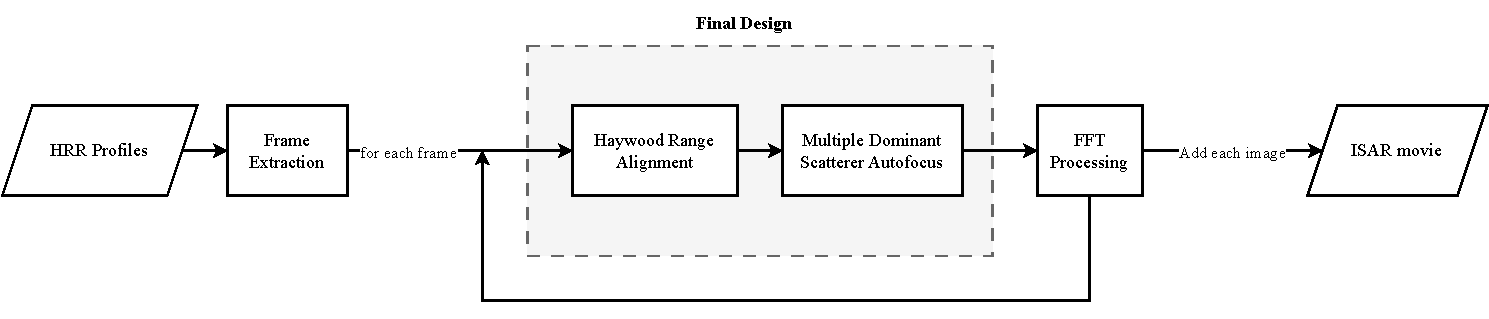
\includegraphics{Figures/05QLPDesign/FlowCharts/QLPDesign.pdf}}
    \caption{Caption}
    \label{fig:enter-label}
\end{figure}

\begin{itemize}
    \item \textbf{Diagram} Flow chart/UML of final system
    \item Link back to user and functional requirements
\end{itemize}
\subsection{App design}
UML DIAGRAM
\begin{itemize}
    \item Link to User requirement of easy use
    \item Show image of app and explain basic functionality and, briefly, design decisions.
\end{itemize}

% ----------------------------------------------------
\ifstandalone
\bibliography{../Bibliography/References.bib}
\printnoidxglossary[type=\acronymtype,nonumberlist]
\fi
\end{document}
% ----------------------------------------------------